\documentclass[aip, jcp, reprint, onecolumn]{revtex4-2}

\bibliographystyle{apsrev4-2}

\usepackage{physics}
\usepackage{amsmath}
\usepackage{amssymb}
\usepackage{mathtools}
\usepackage{graphicx}
\usepackage{dcolumn}
\usepackage[colorlinks=true, linkcolor=black, urlcolor=blue, citecolor=black, anchorcolor=black]{hyperref}

\graphicspath{{"figures/"}}
\begin{document}
%Title of paper
\title{Coherent Hyper-Raman Four Wave Mixing Vibrational Spectroscopies}


\author{Ryan P. McDonnell} 
\author{Daniel D. Kohler}
\author{John C. Wright} \email{wright@chem.wisc.edu}

\affiliation{Department of Chemistry, 
        University of Wisconsin - Madison, 
        Madison, Wisconsin 53706, 
        United States of America}

\date{\today}

\begin{abstract}
Nonlinear, four wave mixing vibrational spectroscopies are often used to probe intramolecular vibrational coupling and relaxation dynamics.
Three wave mixing vibrational spectroscopies are similarly used to understand the spectroscopy and dynamics of interfacial species.
Most of these methods rely on infrared or Raman transitions to generate output. 
Implementing a nonlinear spectroscopy involving hyper-Raman transitions, first appearing under third order perturbation theory, can provide a useful analogue to infrared and Raman based nonlinear spectroscopies to understand the spectroscopy and dynamics of isotropic systems.
Hyper Difference Frequency Generation (HDFG) spectroscopy, also known as singly vibrationally enhanced spectroscopy (SIVE), is an underdeveloped, hyper-Raman based four wave mixing vibrational spectroscopy. 
However, the spectroscopic and dynamic properties of HDFG have not been fully explored.
We derive selection rules for singly resonant hyper-DFG and demonstrate it provides a simpler method to extract hyper-Raman polarizabilities ($\beta$).
HDFG output is shown to be similar in magnitude to vibrational sum frequency generation (vSFG). 
We demonstrate the properties and capabilities of HDFG through measuring spectra and coherence dynamics of multiple infrared active modes in CH$_3$CN.
HDFG shows promise as a method to disentangle ultrafast vibrational dynamics in isotropic systems without need for anharmonicities.

\end{abstract}

\maketitle

\section{Introduction}
Coherent multidimensional spectroscopy (CMDS) is a family of three and four wave mixing methods which form the optical analogue of multidimensional nuclear magnetic resonance (NMR) spectroscopy.\cite{Cho2008, RN335}
Multiresonant, four wave mixing CMDS experiments, first proposed by Oudar and Shen in 1980,\cite{RN307} directly probe coupling between different vibrational, electronic, and vibronic states. \cite{RN307, RN281, RN342, Cho2008, RN335, Ogilvie2019, RN325} 
CMDS has resolved anharmonicities and other intramolecular couplings in numerous systems. \cite{RN345, RN342, RN343, RN324, RN329, RN120, Czech2015, Gaynor2017, Ogilvie2019, RN325}
A particular class of CMDS methods, coherent Raman based four wave mixing spectroscopies, can provide explicit probes of vibrational and excitonic coupling in a variety of systems.

\begin{figure}[!htbp]
	\centering
	\includegraphics[width=3.375in]{dfg_hdfg_hr_wmel.png}
	\caption{Wave Mixing Energy Level (WMEL) diagrams of difference frequency generation (DFG), hyper difference frequency generation (HDFG) and spontaneous hyper-Raman scattering. \cite{RN286, RN352}
		$\ket{g}$ is the ground state, $\ket{v}$ is an infrared active vibration and $\ket{m}, \ket{n}$ are virtual states.
		Solid and dashed horizontal lines indicate real and virtual states, whereas solid and dotted arrows indicate ket and bra side transitions, respectively. %todo: add Raman to this WMEL! dfg Raman hyperDFG hyperRaman 
		}
	\label{fig:comparisonwmel}
\end{figure}

Not all CMDS methods are used to dissect intramolecular couplings.\cite{Shen1987_CPL}
Non-parametric, hyper difference frequency generation (hyper-DFG) spectroscopy, similar to difference frequency generation (\autoref{fig:comparisonwmel}), is a four wave mixing method which, when detuned from  electronic resonances, does not probe intramolecular couplings. 
HDFG was the first infrared CMDS method to successfully discriminate against non-resonant background.\cite{RN351, RN352}
Hyper-DFG has also been referred to as singly vibrationally enhanced (SIVE) spectroscopy. \cite{RN351}
In hyper-DFG, an infrared pulse is resonant with a vibrational mode, and two other input pulses are used to induce a scattering process to provide output.
Hyper-DFG was documented long ago to have characteristics similar to spontaneous hyper-Raman scattering spectroscopy. \cite{RN352}
Hyper-Raman scattering is the two photon analogue to Raman scattering. \cite{Cyvin1965, Terhune1965}
Compared to Raman spectroscopy, hyper-Raman scattering cross sections are often small, making it a difficult technique to successfully implement.\cite{RN515, Kelley2010} 
The different selection rules of hyper-Raman scattering, however, make it a unique alternative to Raman scattering to understand vibrational spectra and vibronic coupling in molecular systems.
In 1998, Cho et al. proposed a parametric six wave mixing technique which was the coherent analogue of hyper-Raman scattering. \cite{Cho1998}
However, since most six wave mixing methods cascade into four wave mixing processes,\cite{RN243, Cho2000_Cascade} it is preferable to investigate coherent four wave mixing analogues to hyper-Raman scattering.

While hyper-DFG showed promise as an upconverted infrared spectroscopy method, it was quickly supplemented by a doubly vibrationally resonant method, doubly vibrationally enhanced (DOVE) spectroscopy, to investigate intra- and intermolecular vibrational coupling. \cite{RN345, RN101, Cho2000}
As a result, investigations of hyper-DFG stagnated; to date, there are less than a dozen studies which report on hyper-DFG. \cite{RN350, RN416, RN351, RN352, RN353, Chen1998, RN362, RN418, Bonn2024, McDonnell2024}
Recent reports highlight non-negligible hyper-DFG interference in DOVE experiments as well as the suitability of hyper-DFG pathways to interpret ultrafast relaxation dynamics in isotropic systems. \cite{Bonn2024, McDonnell2024}
These reports motivate deeper analysis on the properties of hyper-DFG spectroscopy. 

Fully coherent, ultrafast probes of vibronic coupling would yield insight into processes that control ultrafast electronic relaxation in molecular and biological systems. \cite{Bredenbeck2015, Arsenault2021}
Some years ago, Cho proposed a parametric, doubly resonant infrared/visible pathway to probe vibronic coupling in isotropic systems. \cite{Cho2001}
In this method, a single infrared pulse is resonant with a vibrational mode, and a two photon absorption event from a near infrared (NIR) or visible pulse resonant with an electronic or vibronic state is used to generate the four wave mixing signal.
The non-parametric pathways similar to this method are referred to herein as doubly resonant hyper-DFG (DR-HDFG).
Methods analogous to DR-HDFG, where two photon absorption from the infrared pulse and one photon absorption from the visible pulse is used to generate output, i.e., stimulated Raman processes, have been reported. \cite{RN301, RN120} 

An experimental complexity in executing four wave mixing experiments is the demand of three separate input pulses, often all at different frequencies.
For example, in the case of DOVE, two of the three input pulses must be scanable infrared pulses. \cite{RN345} 
Only recently have methods been developed for seamless tuning and scanning of ultrafast optical parametric amplifiers across swaths of frequency space. \cite{RN162, McDonnell2024, SkyeOPA, KyleOPA}
Since HDFG demands only a single resonance to be scanned, the experiment can be performed using two input pulses: one tunable, infrared OPA to scan across vibrational resonances, and a two photon absorption from the signal process of a separate OPA, or output from the oscillator which pumps the infrared OPA.
As such, laboratories experienced in sum frequency generation (SFG) spectroscopy can perform HDFG spectroscopy to understand bulk dynamics and spectroscopy using nearly the same setup.\cite{Shen1987_CPL}

Inspired by recent work which demonstrated the presence of HDFG in ultrafast DOVE experiments,\cite{McDonnell2024} we investigate the parameters which result in both SR and DR-SIVE output. \cite{Cho2000, Bonn2024}
We develop simple expressions which relate transition dipoles and hyper-Raman polarizabilties and the overall HDFG output, yielding gross selection rules. 
It is shown that a HDFG active mode must be both IR and hyper-Raman active.
Since any IR active vibration is also hyper-Raman active, \cite{Andrews1978} we demonstrate that HDFG is a coherent analogue of hyper-Raman scattering spectroscopy for IR active vibrations, i.e., HDFG is an optically upconverted infrared spectroscopy.
This is akin to sum and difference frequency generation (SFG, DFG) being coherent Raman analogues for IR active vibrations. \cite{Shen90}

We investigate properties of DR-HDFG to understand how coupling between vibrational and vibronic states can be measured.
DR-HDFG is shown to demand one and two-photon absorptions between the ground and excited state.
DR-HDFG is thus the four wave mixing analogue of doubly resonant infrared-visible sum frequency generation. \cite{Shen94}

\section{Steady State Hyper-DFG Spectroscopy}
Singly resonant hyper difference generation spectroscopy (HDFG) spectroscopy has potential to provide deeper insight into single quantum decoherence times and molecular orientation in condensed systems.
Similarities between HDFG spectroscopy, infrared spectroscopy and spontaneous hyper-Raman scattering have been noted previously. \cite{RN352, Bonn2024}
In this section, we make the connections between HDFG and hyper-Raman scattering explicit and investigate the steady state properties of singly resonant HDFG.

\begin{figure}[!htbp]
	\centering
	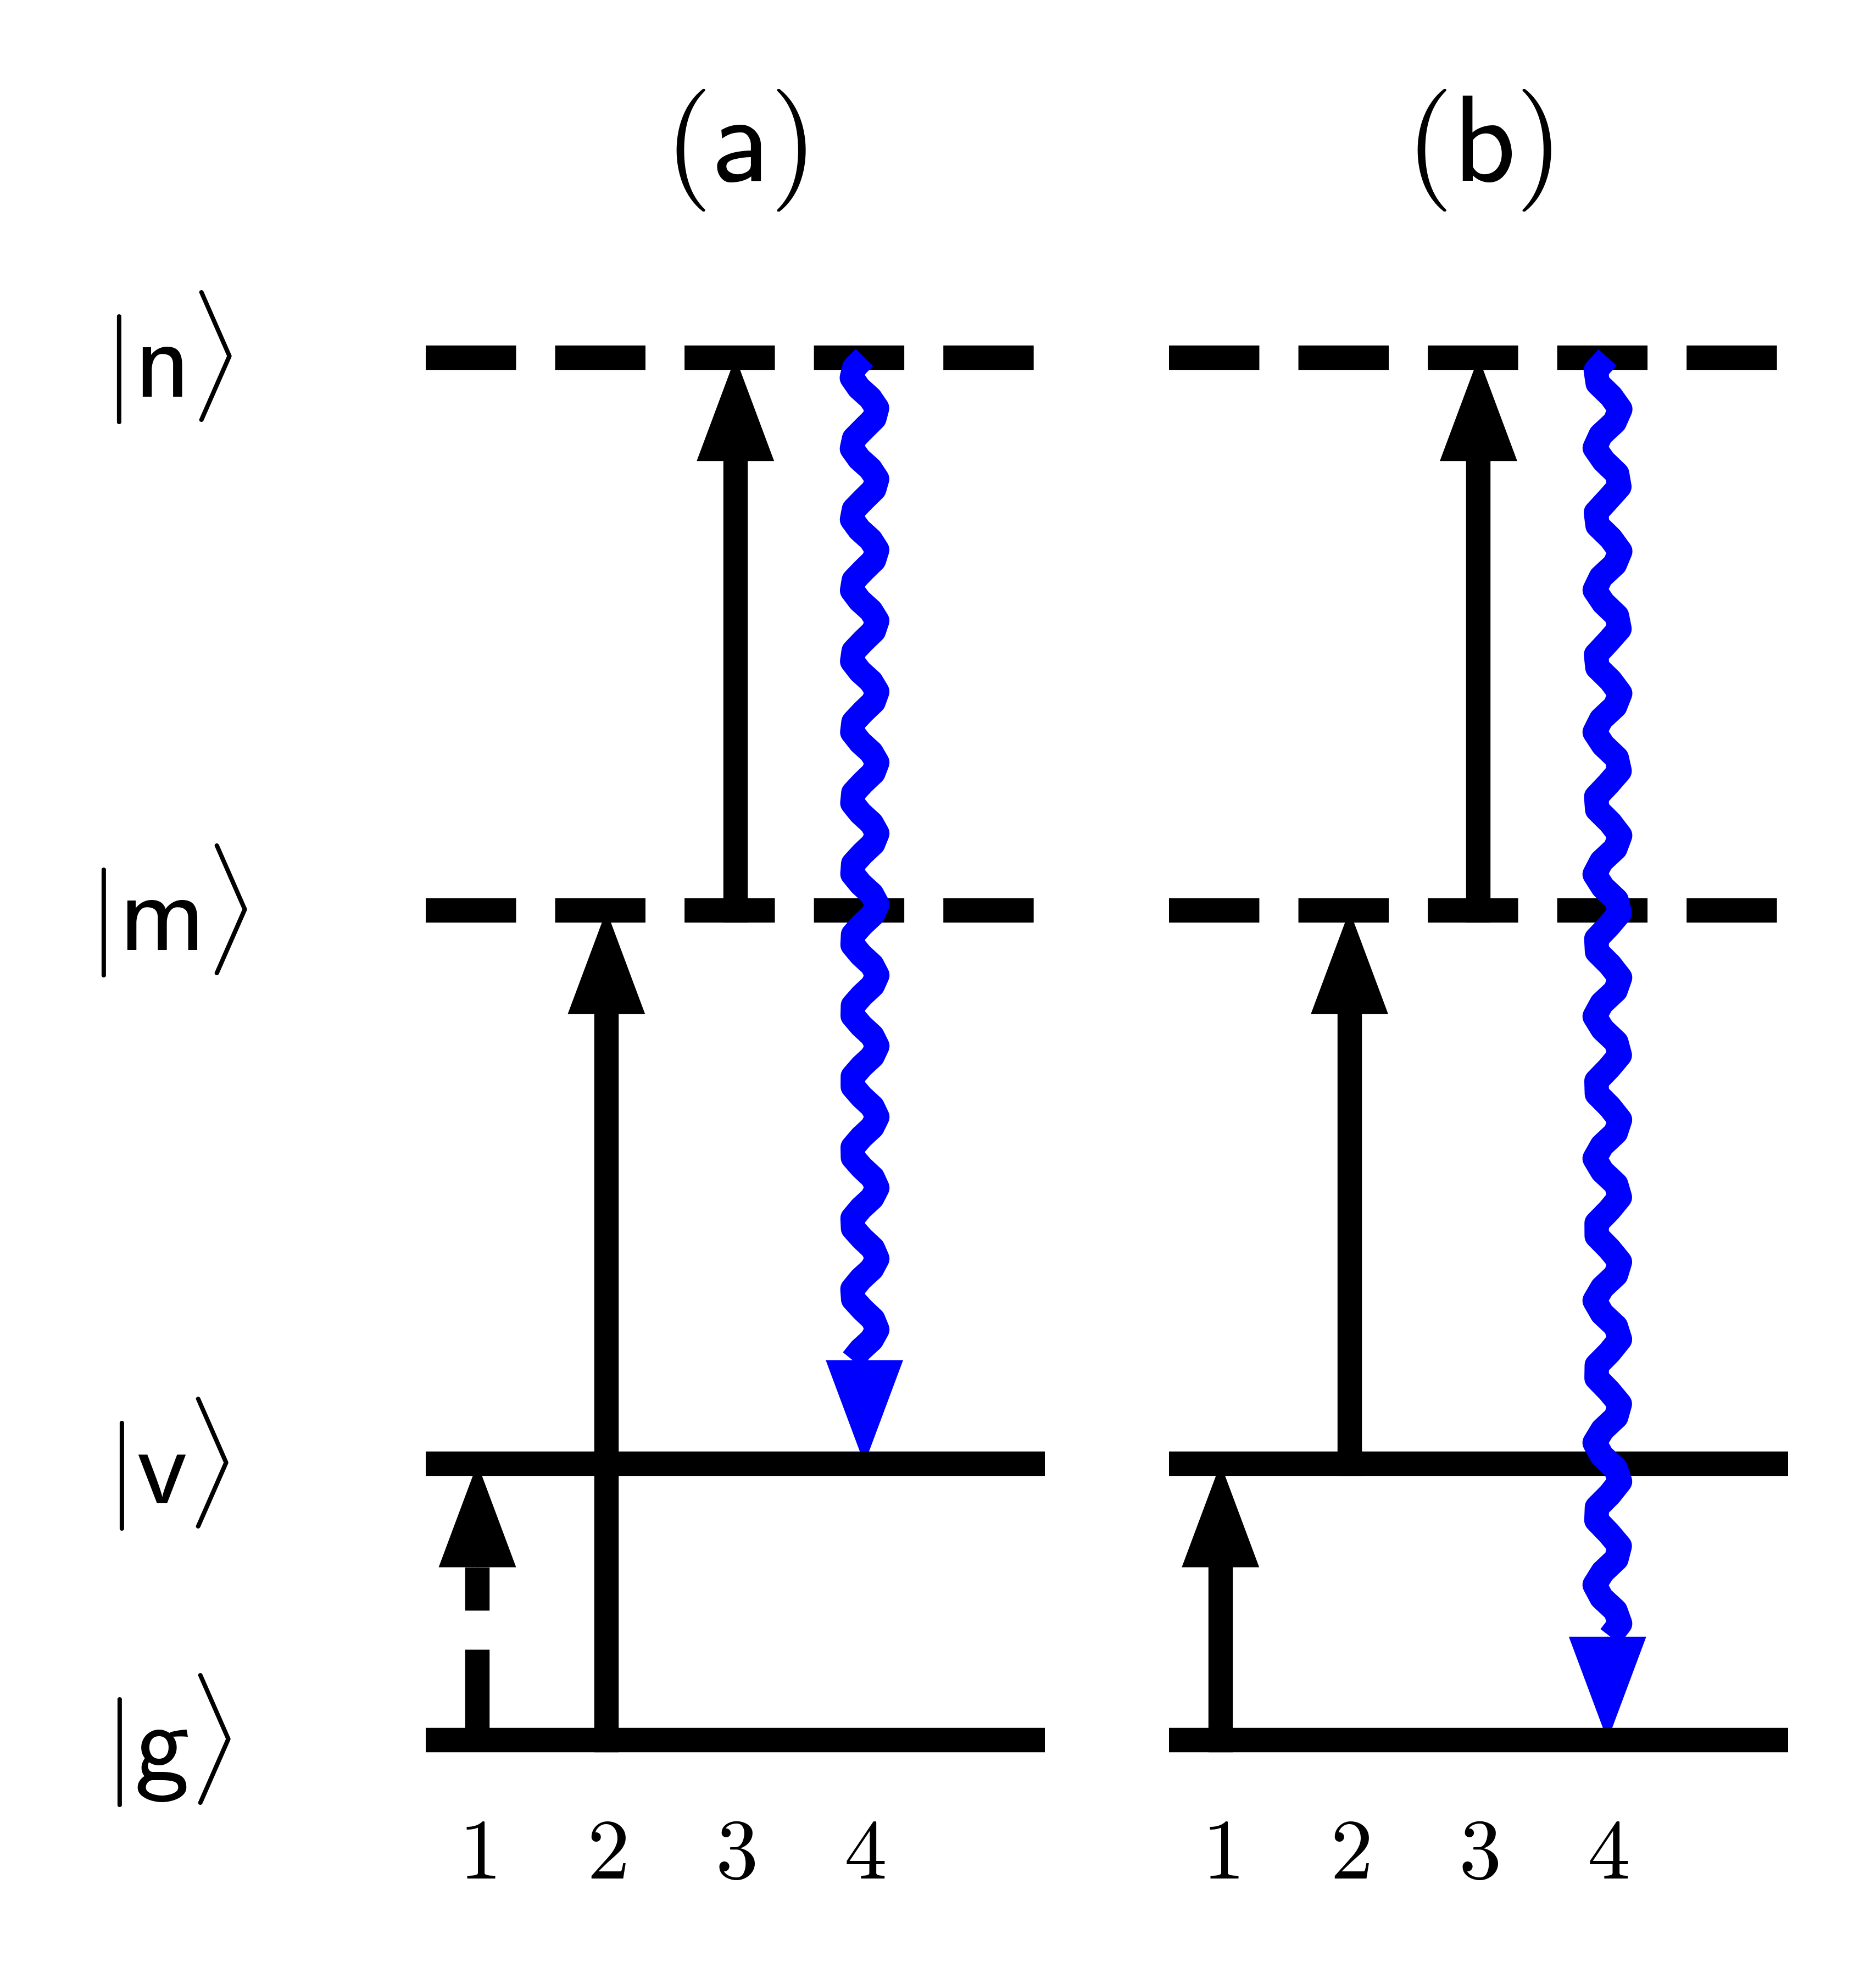
\includegraphics[width=3.375in]{wmel1.png}
	\caption{Wave Mixing Energy Level (WMEL) diagrams of the relevant HDFG pathways in the (a) $\vec{k}_4 = -\vec{k}_1 + \vec{k}_2 + \vec{k}_3$ and (b) $\vec{k}_4 = \vec{k}_1 + \vec{k}_2 + \vec{k}_3$ phasematching geometries. \cite{RN286, RN352}
	$\ket{g}$ is the ground state, $\ket{v}$ is an infrared active vibration and $\ket{m}, \ket{n}$ are virtual states.
	Solid and dashed horizontal lines indicate real and virtual states, whereas solid and dotted arrows indicate ket and bra side transitions, respectively. 
	These diagrams can be permuted to generate additional resonant WMEL diagrams.}
	\label{fig:sivewmel}
\end{figure}

It is useful to expose relationships between transition dipoles, Raman polarizabilities and hyper-Raman polarizabilities in the driven limit. \cite{Simpson2004, RN120}
In the driven limit, under the electric dipole approximation, the I$^{th}$ component of the third order nonlinear output polarization, ${P}^{(3)}_I$, of any four wave mixing process, induced by electric fields E, at output frequency $\omega_4$ is written as \cite{RN307}
\begin{equation} \label{polarization}
{P}^{(3)}_I (\omega_4)  = \chi^{(3)}_{IJKL} E_J E_K E_L 
\end{equation}
where $\chi^{(3)}_{IJKL}$ is the IJKL element of the third order electrical susceptibility, a rank four tensor, generally written as
\begin{equation}
	\chi^{(3)}_{IJKL} = NF(\omega_4) \langle \gamma_{ijkl} \rangle
\end{equation}
where N is a number density, F is the Lorentz local field factor, and $\gamma_{ijkl}$ is the third order polarizability (i.e., second hyperpolarizability). 
The brackets indicate an orientational average. 
Uppercase letters refer to laboratory frame coordinates and lower case letters refer to molecular frame coordinates.

To make the connection between HDFG and hyper-Raman scattering, we investigate its gross selection rules.
By propagating density matrix elements in the steady state limit, the HDFG hyperpolarizability is \cite{RN119}
\begin{equation}\label{sivegamma}
		\gamma_{ijkl} =	- \sum_{m, n} \frac{1}{\varepsilon_0} \frac{1}{4D} \frac{1}{\hbar^3} \frac{\mu^{i}_{v n} \mu^{j}_{nm} \mu^{k}_{mg} \mu^{l}_{gv} }{\Delta_{nv} \Delta_{mv}\Delta_{gv}}  \rho_{gg}
\end{equation}
where: $\mu^{j}_{ab}$ is the $j^{th}$ element of $\mel{a}{\vec{\mu}}{b}$, $\Delta_{kl} = \omega_{kl} - \omega_{j} - i\Gamma_{kl}$, $\omega_j$ is the frequency of the j$^{th}$ input field, $\Gamma_{kl}$ is the dephasing of $\rho_{kl}$ and $\rho_{gg}$ is the ground state population.
For simplicity, we consider the results for the process diagrammed in \autoref{fig:sivewmel}a, but by multiplying by (-1) and taking a complex conjugate, which arise from the bra-side transition in \autoref{fig:sivewmel}a, results for the \autoref{fig:sivewmel}b  process are obtained.
Note that $\omega_j \rightarrow -\omega_j$ for a bra side transition.
D, the Maker-Terhune degeneracy factor, accounts for permutation symmetry in $\gamma_{ijkl}$ and is defined as $\frac{n!}{(n-m)!}$, where $n$ is the total number of input fields (3 for any four wave mixing experiment) and $m$ is the number of distinguishable input fields.\cite{RN134} 
For a HDFG experiment using two or three distinct input fields, as considered here, D = 6.
Note that $\ket{m}, \ket{n}$ are virtual states (\autoref{fig:sivewmel}).
By contracting over the virtual states to form the hyper-Raman hyperpolarizability $\beta$ (i.e., Placzek approximation), this expression can be simplified immensely.\cite{Long1970} 
Note, however, that if $\omega_2$, $\omega_3$, as depicted in \autoref{fig:sivewmel}, are nearly resonant with any state, the Placzek approximation fails. \cite{Placzek1934, Long1970}
Assuming the validity of the Placzek approximation, \autoref{sivegamma} is written as 
\begin{equation}\label{sivebeta}
	\gamma_{ijkl} =	-\frac{1}{\varepsilon_0} \frac{1}{24 \hbar}\frac{\beta^{(ijk)}_{gv} \mu^{(l)}_{gv}}{\Delta_{gv}} \rho_{gg}
\end{equation}
Taylor expanding the dipole and first hyperpolarizability operators in terms of an n$^{\text{th}}$ normal mode coordinate $Q_n$ about equilibrium: \cite{Long1970}
\begin{subequations}
	\begin{equation}
		\mu = \mu_0 + \frac{\partial \mu}{\partial Q_n} Q_n + \order{{Q_m Q_n}}
	\end{equation}
	\begin{equation}
		\beta = \beta_{0} + \frac{\partial \beta}{\partial Q_n} Q_n + \order{{Q_m Q_n}}
	\end{equation}
\end{subequations}
Substituting into \autoref{sivebeta}, and knowing that $\mel{v}{Q_n}{g} = \sqrt{\frac{\hbar}{2m_n\omega_{vg}}}$ under the harmonic approximation,\cite{RN230} where $m_n$ is the mass of the $Q_n$ mode, gives the HDFG hyperpolarizability to $\order{Q_n}$ as \begin{equation}\label{SIVEselection}
	\gamma_{ijkl} =	-\frac{1}{\varepsilon_0} \frac{1}{48 m_n \omega_{vg}}  \frac{1}{{\Delta_{gv}}} \ \frac{\partial \beta^{(ijk)}}{\partial Q_n} {\frac{\partial \mu^{(l)}}{\partial Q_n}}  \rho_{gg}
\end{equation}
Since this expression is non-zero in the harmonic oscillator limit, HDFG output is allowed for harmonic transitions. 
Similar to SFG, HDFG does not demand anharmonic ground state potential energy surfaces for spectral output. \cite{Shen94, Cho2000}
This selection rule is generally valid for any HDFG or hyper sum frequency generation (HSFG) process in the $-\vec{k}_1 + \vec{k}_2  + \vec{k}_3$ and $\vec{k}_1 + \vec{k}_2  + \vec{k}_3$ phasematching geometries when the Placzek approximation is valid.

\autoref{SIVEselection} shows any HDFG active mode must be both hyper-Raman and IR active.
However, since any IR active vibrational mode is hyper-Raman active,\cite{Cyvin1965, Andrews1978} any IR active mode is HDFG active.
This makes HDFG an optically upconverted infrared spectroscopy of isotropic samples, as its selection rules are identically those of IR spectroscopy, but its output is generally in the visible.
A useful attribute of the $\beta_{ijk}$ dependence in HDFG output is added polarization control. 
Similar to SHG and SFG experiments that probe different elements of the infrared transition dipole and Raman polarizability tensors,\cite{Heinz1982} probing different elements of $\beta_{ijk}$ in HDFG can greatly assist in understanding ultrafast dynamics in isotropic systems, as suggested by Seliya et al. \cite{Shen90, Bonn2024}
Polarization control in IR-pump-HDFG-probe, analogous to ultrafast transient absorption spectroscopy for vibrational modes, would be an interesting venue to assess the sensitivity of HDFG to different hyper-Raman tensor elements. 


Previous spontaneous hyper-Raman work interpreted the origin of hyper-Raman signal in terms of Franck-Condon, Herzberg-Teller and Duschinsky type couplings.\cite{Ziegler1988} %todo: cite the other papers.
As such, we investigate \autoref{SIVEselection} using an Albrecht ABC type formalism which naturally incorporates these types of couplings.
To do so, we write the states in terms of a Born-Oppenheimer basis $\ket{a,b}$, where $\ket{a,b} = |a) \otimes \ket{b}$ for electronic states $\{|a)\}$ and vibrational states $\{\ket{b}\}$. \cite{BornOppenheimer, Albrecht1960}
Here, $\ket{g}, \ket{v}$ are vibrational states on the ground electronic state $|g)$ and $\ket{m} \rightarrow \ket{m,j}$, $\ket{n} \rightarrow \ket{n,k}$ are virtual states.
For consistency with previous reports, we use $\vec{R}$ to denote electric transition dipole moments ($\vec{\mu}$ is used for transitions between states on the ground electronic state.). \cite{Ziegler1974}
Following the approach which gave \autoref{sivegamma}, we find
\begin{equation}\label{drgamma_notaylor}
	\gamma_{ijkl} = -\frac{1}{\varepsilon_0} \frac{1}{24 \hbar^3} \sum_{m,n,j,k} \frac{
		R^{i}_{gv, nk} 
		R^{j}_{nk,mj} 
		R^{k}_{mj,gg} 
		R^{l}_{gv,gg} 
	}{\Delta_{g0,gg}
		\Delta_{nk, mj}
		\Delta_{mj, gg}
	}
\end{equation}
where $R^{i}_{ab,cd}$ is the i$^{th}$ element of $\mel{a,b}{\vec{R}}{c,d}$.\cite{Ziegler1988}
Using our definition of vibronic states, we write $\vec{M}_{ab} = (a|\vec{M}|b)$ so that, for example,
$R^{i}_{gv,ev'} = \mel{v}{M^i_{ge}}{v'}$.\cite{Albrecht1960}
Using these ideas rewrites \autoref{drgamma_notaylor} as
\begin{equation}\label{drgamma_notaylor_1}
	\begin{split}
		\gamma_{ijkl} &= -\frac{1}{\varepsilon_0} \frac{1}{24 \hbar^3} \sum_{m,n,v'} \frac{
			\mel{v}{M^{i}_{ge}}{v'} 
			\mel{v'}{M^{j}_{em}}{n}
			\mel{n}{M^{k}_{mg} }{v}
			\mel{v}{M^{l}_{gg}}{0}
		}{\Delta_{g0,gv}
			\Delta_{ev', mn}
			\Delta_{mn, g0}	} \\
	\end{split}
\end{equation}
Chung and Ziegler showed some years ago that expanding ${\vec{M}_{ij}}$ to $\order{Q}$ yields $A, B, C$ coefficients similar to the Albrecht formalism of Raman scattering. \cite{Albrecht1961, Ziegler1988}
The $A$ term depends upon Franck-Condon $\order{Q^0}$ transitions, the $B$ term depends upon Herzberg-Teller ($\order{Q}$) transitions, and the $C$ term depends on Duschinsky ($\order{Q^2}$) transitions. 
Here, we ignore the C term as it depends on one and two photon forbidden transitions which have yet to be observed in spontaneous hyper-Raman scattering. \cite{Ziegler1988}
The full derivation of $A,B$ have been given elsewhere, so only their final forms will be given.

By compiling all the terms that scale with $\order{Q^0}$, i.e. $\vec{M}_{ij_0}$, $A$ is written as
\begin{equation}
	\begin{split}
		A_{ijk} &= \text{crap times Franck Condon}\\
	\end{split}
\end{equation}
where terms such as $\langle v | v' \rangle$ are Franck-Condon factors.

something about the A term. SHOW THAT IT VANISHES FOR SINGLY RES TERMS

It is important to note that in the case of singly resonant HDFG, $A_{ijk}$ vanishes, or only Herzberg-Teller contributions are present in SR-HDFG. \cite{Neddersen1989}

Similarly, the $B$ terms scale with $\order{Q}$, such that
\begin{equation}
	\begin{split}
		B_{ijk} &= \text{crap}\\
	\end{split}
\end{equation}
Then B term. 
B term has new sum over another normal mode Ql that must be included because when I expand in terms of Q there are 3N-6-1 normal modes I can talk to (3N-6-1, assuming nonlinear and that the -1 comes from assuming we end in v)
Blah Blah Blah
%todo: So clearly HDFG has heavy dependence on HT type couplings! 
%This likely explains the relative weakness of HDFG in solvents such as hexane. \cite{RN351}
%fix the equation so that the dipole is clearly isolated from the hyper Raman part. Write beta as A+B+C?
%todo: segue into vibronic coupling

While HDFG can provide useful information about the properties of molecular vibrations, it is immediately apparent that \autoref{fig:sivewmel} can inform on molecular electronic structure by making the hyper-Raman transition resonant with a vibronic state.
DR-HDFG (where a vibrational and vibronic state are resonantly coupled) can provide a tool for measuring vibronic coupling.
This method is analogous to doubly resonant sum frequency generation (DR-SFG). \cite{Shen94}
Many multi-resonant nonlinear spectroscopies have been developed to resolve vibronic coupling in molecular samples. \cite{Carlson1990, Gaynor2017, RN276}
DR-HDFG provides methods to investigate vibronic coupling with only two laser pulses, as long as the electronic state is accessible via two photon absorption from the ground state (\textit{vide infra}).
Two beam, parametric and non-parametric DR-HDFG processes are diagrammed in \autoref{fig:doubsive}.
%todo: insert discussion on ABC terms
%todo: write hamiltonian like Gaynor to make clear what we are doing (and put in a picture in Figure doubbleresspec)

To interpret HDFG selection rules, we use a slightly modified version of equation xyz to account for the added vibronic resonance. 
This change immediately makes the A term nonzero in the case of noncentrosymmetric systems.

A simulated spectrum highlighting the contributions of these terms (\autoref{fig:doubres_spec}) on potential wells with displacements $\Delta$ shows... 
\begin{figure}[!htbp]
	\centering
	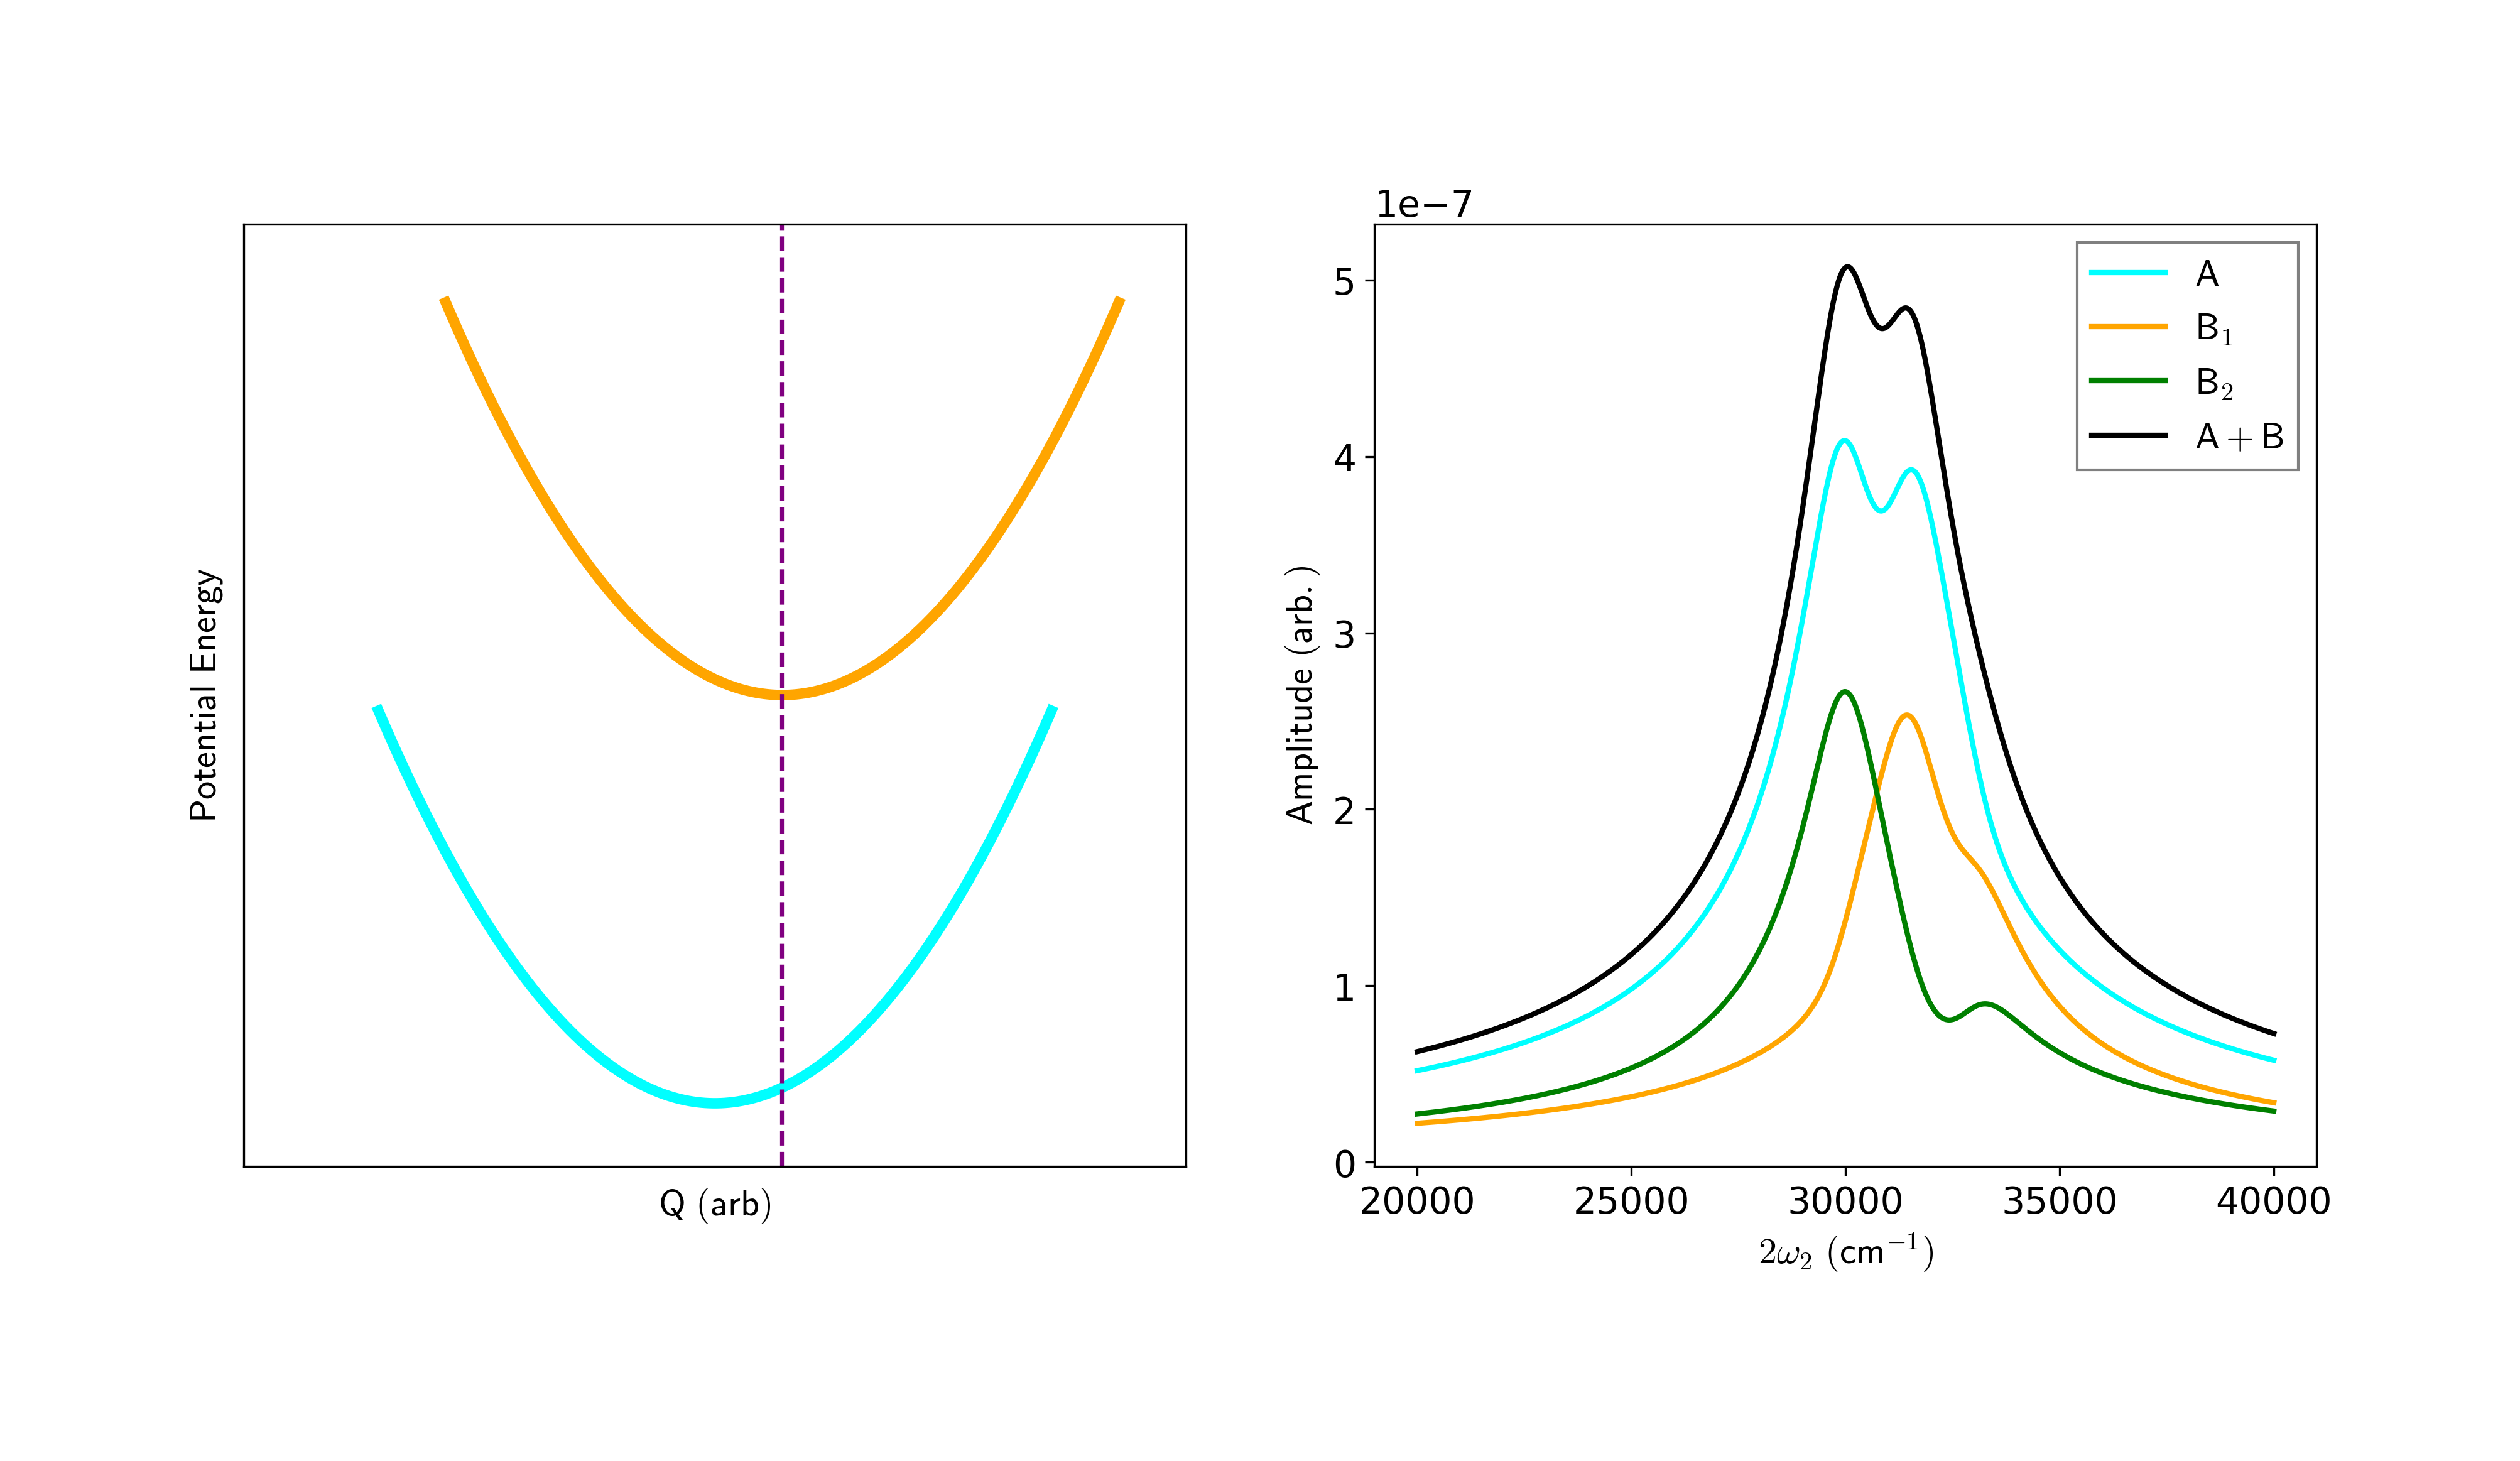
\includegraphics[width=3.375in]{drsive_spectrum.png}
	\caption{Spectrum showing sensitivity of DR-HDFG to well displacements in vibronic coupling.
		Model includes both Franck-Condon and Herzberg Teller effects.
		(a) Potential energy surfaces, 2D spectrum where (b) $\Delta = 0$, (c) $\Delta = 0.5$, (d) $\Delta = 1$}
	\label{fig:doubres_spec}
\end{figure}

%These results also make DR-HDFG a type of resonance IR spectroscopy, as introduced by Boyle et al for resonant triple sum frequency generation.\cite{RN491} 
%However, in the methods described by \autoref{drgamma_alpha_0}, $|e)$ must be accessible through one and two photon transitions from $|g)$.
%Conversely, the resonance-IR method demonstrated by Boyle et al. only requires one photon transitions between $|g)$ and $|e)$.
%Systems which provide strict parity selection rules (e.g., benzene) will be useful for assessing the validity of these selection rules and comparing the method described here and that of Boyle et al. \cite{RN491}




\subsection{Quantification}
Since the hyper-Raman process is stimulated by a two-photon process, a setup using only two lasers can perform a coherent four wave mixing hyper-Raman experiment by investigating $\pm \vec{k}_1 + 2\vec{k}_2$ processes, assuming a two photon absorption from a single pulse stimulates the hyper-Raman process.
The other commonly used two laser CMDS method is sum frequency generation, a $\chi^{(2)}$ technique, whose phasematching is dictated by $\vec{k}_1 + \vec{k}_2$.
The SFG output scales as $\chi^{(2)}_{IJK} \sim \langle \alpha_{ij} \mu_k \rangle$, where $\alpha_{ij}$ is the Raman polarizability tensor.
Since SFG is dependent upon transitions that transform like both rank-one and rank-two tensors, this enforces a microscopic constraint that SFG cannot yield output for centrosymmetric species under the electric dipole approximation.
This follows from the presence of an inversion center in centrosymmetric systems, which demands strict parity selection rules. \cite{RN230}
Macroscopically, inversion symmetry in the output polarization eliminates output from centrosymmetric species under the electric dipole approximation.\cite{RN227, RN132}
As a result, the output of SFG is significantly reduced relative to most third order spectroscopies because the output only depends on surface species.
However, since HDFG is dependent upon a hyper-Raman transition, it is useful to compare the relative output of the two processes to identify how HDFG output compares to SFG.

To motivate the application of HDFG spectroscopy, we perform a calculation to compare HDFG and vibrational SFG (vSFG) output.
Absorption effects are neglected for simplicity.
\begin{widetext}
To allow comparison between the two methods, the output polarizations of each process is written as
	\begin{subequations}
		\begin{equation}
			\abs{P^{(2)}_{\text{SFG}}} = N_{surf} F(\omega_1+\omega_2) \abs{\langle \alpha_{ij}\mu_{k} \rangle E_J(\omega_2)E_K(\omega_1)} 
		\end{equation}
		\begin{equation}
			\abs{P^{(3)}_{\text{HDFG}}} = N_{bulk}  F(-\omega_1+\omega_2 +\omega_3) \abs{\langle \beta_{ijk} \mu_{l} \rangle E_J{(\omega_3)}E_K(\omega_2)E_L(-\omega_1)} \ell_{eff}
		\end{equation}
	\end{subequations}
where N$_{bulk}$ is the bulk number density, and N$_{surf}$ is the surface number density (10$^{19}$ m$^{-2}$).\cite{RN133, RN503}	
For liquids with molar masses less than $\sim$100 g mol$^{-1}$ and densities roughly equal to that of H$_2$O$_{(l)}$ at room temperature, N$_{bulk} \sim$ 10$^{28}$ m$^{-3}$.
We take the bulk optical interaction length ($\ell_{eff}$) to be 10 $\mu$m.\cite{RN133} %see chapter 25 of Shen's NLO book... idk something here seems wrong
A normal dispersion curve is assumed so that $F(\omega_1+\omega_2) \approx F(-\omega_1+\omega_2 +\omega_3)$.
To simplify analysis, orientational averaging is ignored (e.g., $\langle \beta_{ijk} \mu_{l} \rangle \approx \beta \mu$) and the input and output fields are taken to be co-polarized, so that
\begin{equation}
		P_{ratio} \equiv \frac{\abs{P^{(3)}_{\text{HDFG}}}}{\abs{P^{(2)}_{\text{SFG}}}} \approx \frac{N_{bulk}}{N_{surf}} \frac{\beta}{\alpha} E(\omega_3) \ell_{eff} \sim 10^4 \frac{\beta}{\alpha} E(\omega_3)\\
\end{equation}
\end{widetext}
Ziegler has noted that for a field of intensity 10 GW/cm$^{2}$, $\frac{\beta E}{\alpha} \sim 10^{-3} $ for vibrational modes when $E(\omega_3)$ is largely detuned from electronic resonances. \cite{RN515}
Such an intensity is easily obtained using modern ultrafast sources.
In this limit, $P_\text{ratio} \sim 10$.
Since the intensity ratio scales as $\abs{P_{ratio}}^2$, we see that the HDFG output is somewhat stronger than vibrational SFG, assuming only interfacial contributions in vSFG.
It is important to note that this derivation ignored absorption and orientational averaging effects, which can significantly reduce output from either process. 

With the selection rules of HDFG understood for vibrational spectroscopy, it becomes possible to extract quantitative information from its spectra.
Lineshape analysis is essential for extracting quantitative information from CMDS spectra.
Scanning across resonances create dispersive lineshapes, i.e, self-heterodyning, which inform on $\Re(\chi^{(3)})$ and $\Im(\chi^{(3)})$.\cite{Levenson1974_1, Levenson1974_2}
In the method introduced by Levenson and Bloembergen (Bloembergen Interferometry Experiment), an internal standard interferes with the resonant lineshape.
The internal standard is often chosen to be C$_6$H$_6$ or C$_6$D$_6$, due to the strong Raman activity and measured $\chi^{(3)}$ of its ring breathing mode ($\nu_2$ in Herzberg notation). \cite{Levenson1974_2, RN351, RN345}
%okay clearly this wont work lol we need something that is IR active... CaF2?%
Self-heterodyning of the internal standard signal measures $\chi^{(3)}$ and does not require measurement of absolute intensities. 
Resonant lineshapes are also complicated by amplitude level interference between the sample and its substrate and/or sample cell windows, which must be accounted for to obtain quantitatively correct $\chi^{(3)}$ values. \cite{RN362, RN418}

Most quantitative methods in an n$^{th}$ order CMDS experiment are used to extract $\chi^{(n)}$ values to compare the relative strength of nonlinear processes in different media. \cite{Zhu87, RN351, RN345}
The recorded $\chi^{(n)}$ values provide insight into how microscopic quantities ($\vec{\mu}, \alpha_{ij}, \beta_{ijk}$) impact nonlinear output.
To our knowledge, only vibrational SFG and 2D-IR spectroscopy has taken advantage of orientationally averaged $\chi^{(n)}$ values to extract transition moments. \cite{Shen90, Moilanen2009, RN245}
It is thus useful to investigate how a simple treatment of orientational averaging can extract $\beta_{ijk}$ from $\chi^{(3)}_{IJKL}$.

The HDFG $\chi^{(3)}_{IJKL}$ expression is
\begin{equation}\label{chi3}
\begin{split}
		\chi^{(3)}_{IJKL} &= NF(\omega_4) \langle \gamma_{ijkl} \rangle = -\frac{NF}{24 \hbar \varepsilon_0 \Delta_{gv}} \langle \beta_{ijk} \mu_l \rangle \rho_{gg}\\
\end{split}
\end{equation}
This expression cannot be used as written to extract $\beta_{ijk}$, as $\beta_{ijk}$ is a Hermitian operator, but $\Delta_{gv} \in \mathbb{C}$. 
However, since the real and imaginary parts of $\chi^{(3)}$ can be extracted from the Bloembergen interferometry experiment, and $\beta_{ijk}$ is present in either term, we can choose to focus on the real or imaginary part of $\chi^{(3)}$.
For simplicity, we investigate $\Im(\chi^{(3)})$, giving, assuming resonance conditions, 
\begin{equation}
	\langle \beta_{ijk} \mu_{l} \rangle = \frac{24 \hbar \varepsilon_0}{NF} \Gamma_{gv} \frac{1}{\rho_{gg}} \Im(\chi^{(3)}_{IJKL})
\end{equation}

The steps behind orientational averaging of $\gamma_{ijkl}$, a rank four tensor in the molecular frame, are detailed elsewhere.\cite{Andrews1977, McDonnell2024}
Orientational averaging shows specific polarization schemes isolate linear combinations of different $\beta_{ijk}$ terms. 
Infrared spectra can provide $\vec{\mu}$ values.
Since $\vec{\mu}$ is a rank-one tensor, its three Cartesian components share the simple relationship $\langle {\mu^2_x} \rangle = \langle {\mu^2_y} \rangle = \langle {\mu^2_z} \rangle = \frac{1}{3}\langle {\mu^2} \rangle$. \cite{RN459}
Neglecting rotational dependence (i.e., assuming only vibrational transitions), $\langle {\mu^2} \rangle = \mu^2$, so that $\langle \beta_{ijk} \mu_l \rangle = \langle \beta_{ijk} \rangle \frac{\abs{\mu}}{\sqrt{3}}$.
By introducing the reduced mass coordinate $q_n = \sqrt{\frac{1}{m_n}} Q_n$ and using the expansions of $\beta_{ijk}$ and $\mu_{l}$ to $\order{Q_n}$ found earlier, we see
\begin{equation}\label{betasive}
	\langle \frac{\partial \beta_{ijk}}{\partial q_n} \rangle = \varepsilon_0 \frac{48 \sqrt{3} }{NF}  \frac{\Gamma_{gv} \omega_{vg}}{\rho_{gg}} \frac{\Im(\chi^{(3)}_{IJKL})}{\frac{\partial \mu}{\partial q_n}}
\end{equation}
Since $\abs{\mu}$ values can be readily extracted from FT-IR spectra,\cite{RN412} this shows that HDFG can give quantitative information on the magnitude of $\beta_{ijk}$.
HDFG and vSFG together provide unique methods to extract the microscopic quantities ($\mu, \alpha, \beta$) that drive nonlinear output.

\begin{figure}[!htbp]
	\centering
	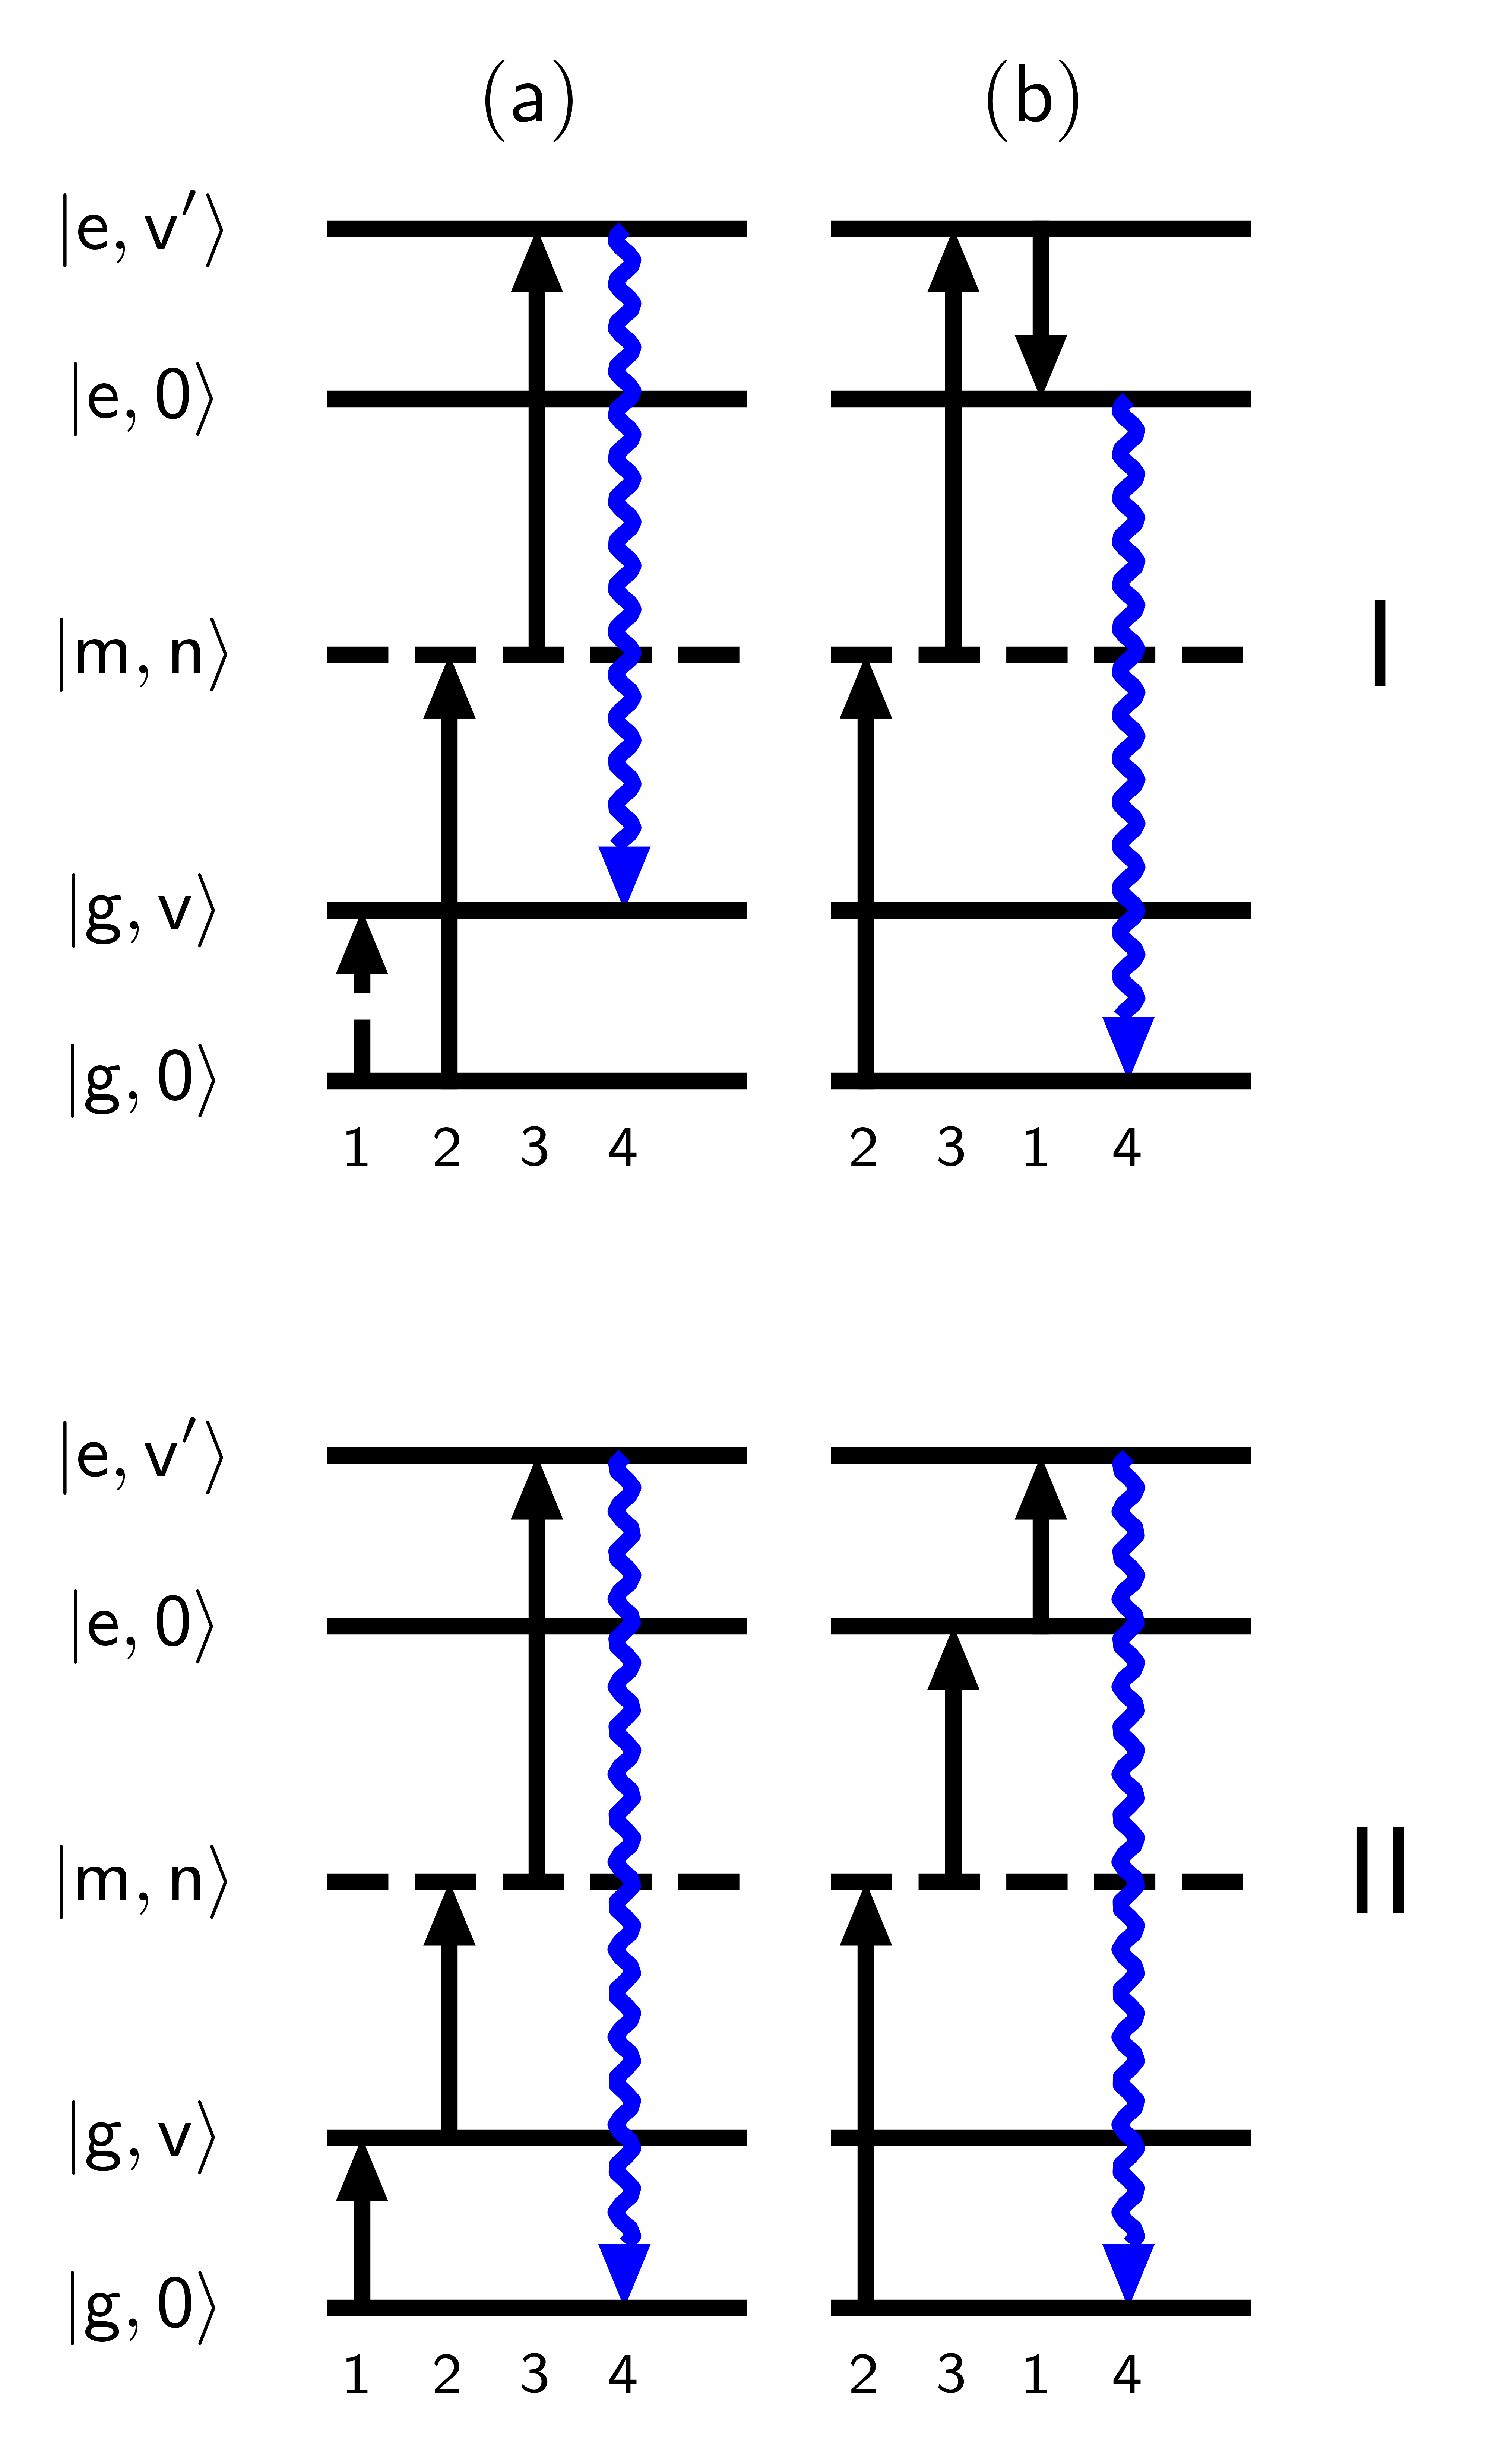
\includegraphics[width=3.375in]{wmel3.png}
	\caption{WMEL diagrams of some (I-a,I-b) DR-HDFG and (II-a,II-b) DR-HSFG pathways. $\ket{g,0}$ denotes the ground states, $\ket{g,v}$ denotes a vibrational state on the ground electronic manifold; $\ket{m,n}$ denotes a virtual state, and $\ket{e,0}, \ket{e,v'}$ denote vibronic states.}
	\label{fig:doubsive}
\end{figure}



\subsection{Comparison to 2DEV and 2DVE spectroscopy}
Compare James' stuff and make connections.


\section{Mixed-Domain Hyper-DFG}
Some words about why mixed domain is great (kill NRB, isolate FID based stuff etc)
Then introduce problems (pathway interference) which can screw things up. This then leads into the main section.

It is well known that nonlinear wave mixing processes which share the same time ordering and output frequency will interfere. \cite{RN135, Bonn2024}
Understanding interfering pathways is useful because they can, in some cases, eliminate output. \cite{RN342, RN135}
The WMEL diagrams presented in \autoref{fig:sivewmel} outline resonant HDFG processes when the infrared pulse $(\omega_1)$ is resonant with a vibrational mode. 
However, if $\omega_2$ ($\omega_1$) becomes resonant (non-resonant), then other HDFG pathways appear.\cite{McDonnell2024} 
While the methods in \autoref{fig:sivewmel2} possess identical selection rules to \autoref{fig:sivewmel}, the WMEL diagrams presented in \autoref{fig:sivewmel2} may significantly interfere with DOVE-IR and DOVE-Raman spectra.
The time ordering in DOVE-IR and DOVE-Raman spectra is used to interpret anharmonicities, as DOVE-IR and DOVE-Raman destructively interfere when outputs are at the same frequency. \cite{RN135, RN324}
It is therefore important to understand how the corresponding HDFG pathways interfere.
To this end, we investigate how the HDFG-IR-II and HDFG-Raman pathways (\autoref{fig:sivewmel2}a, b, respectively) interfere under the rotating wave approximation. 

\begin{figure}[!htbp]
	\centering
	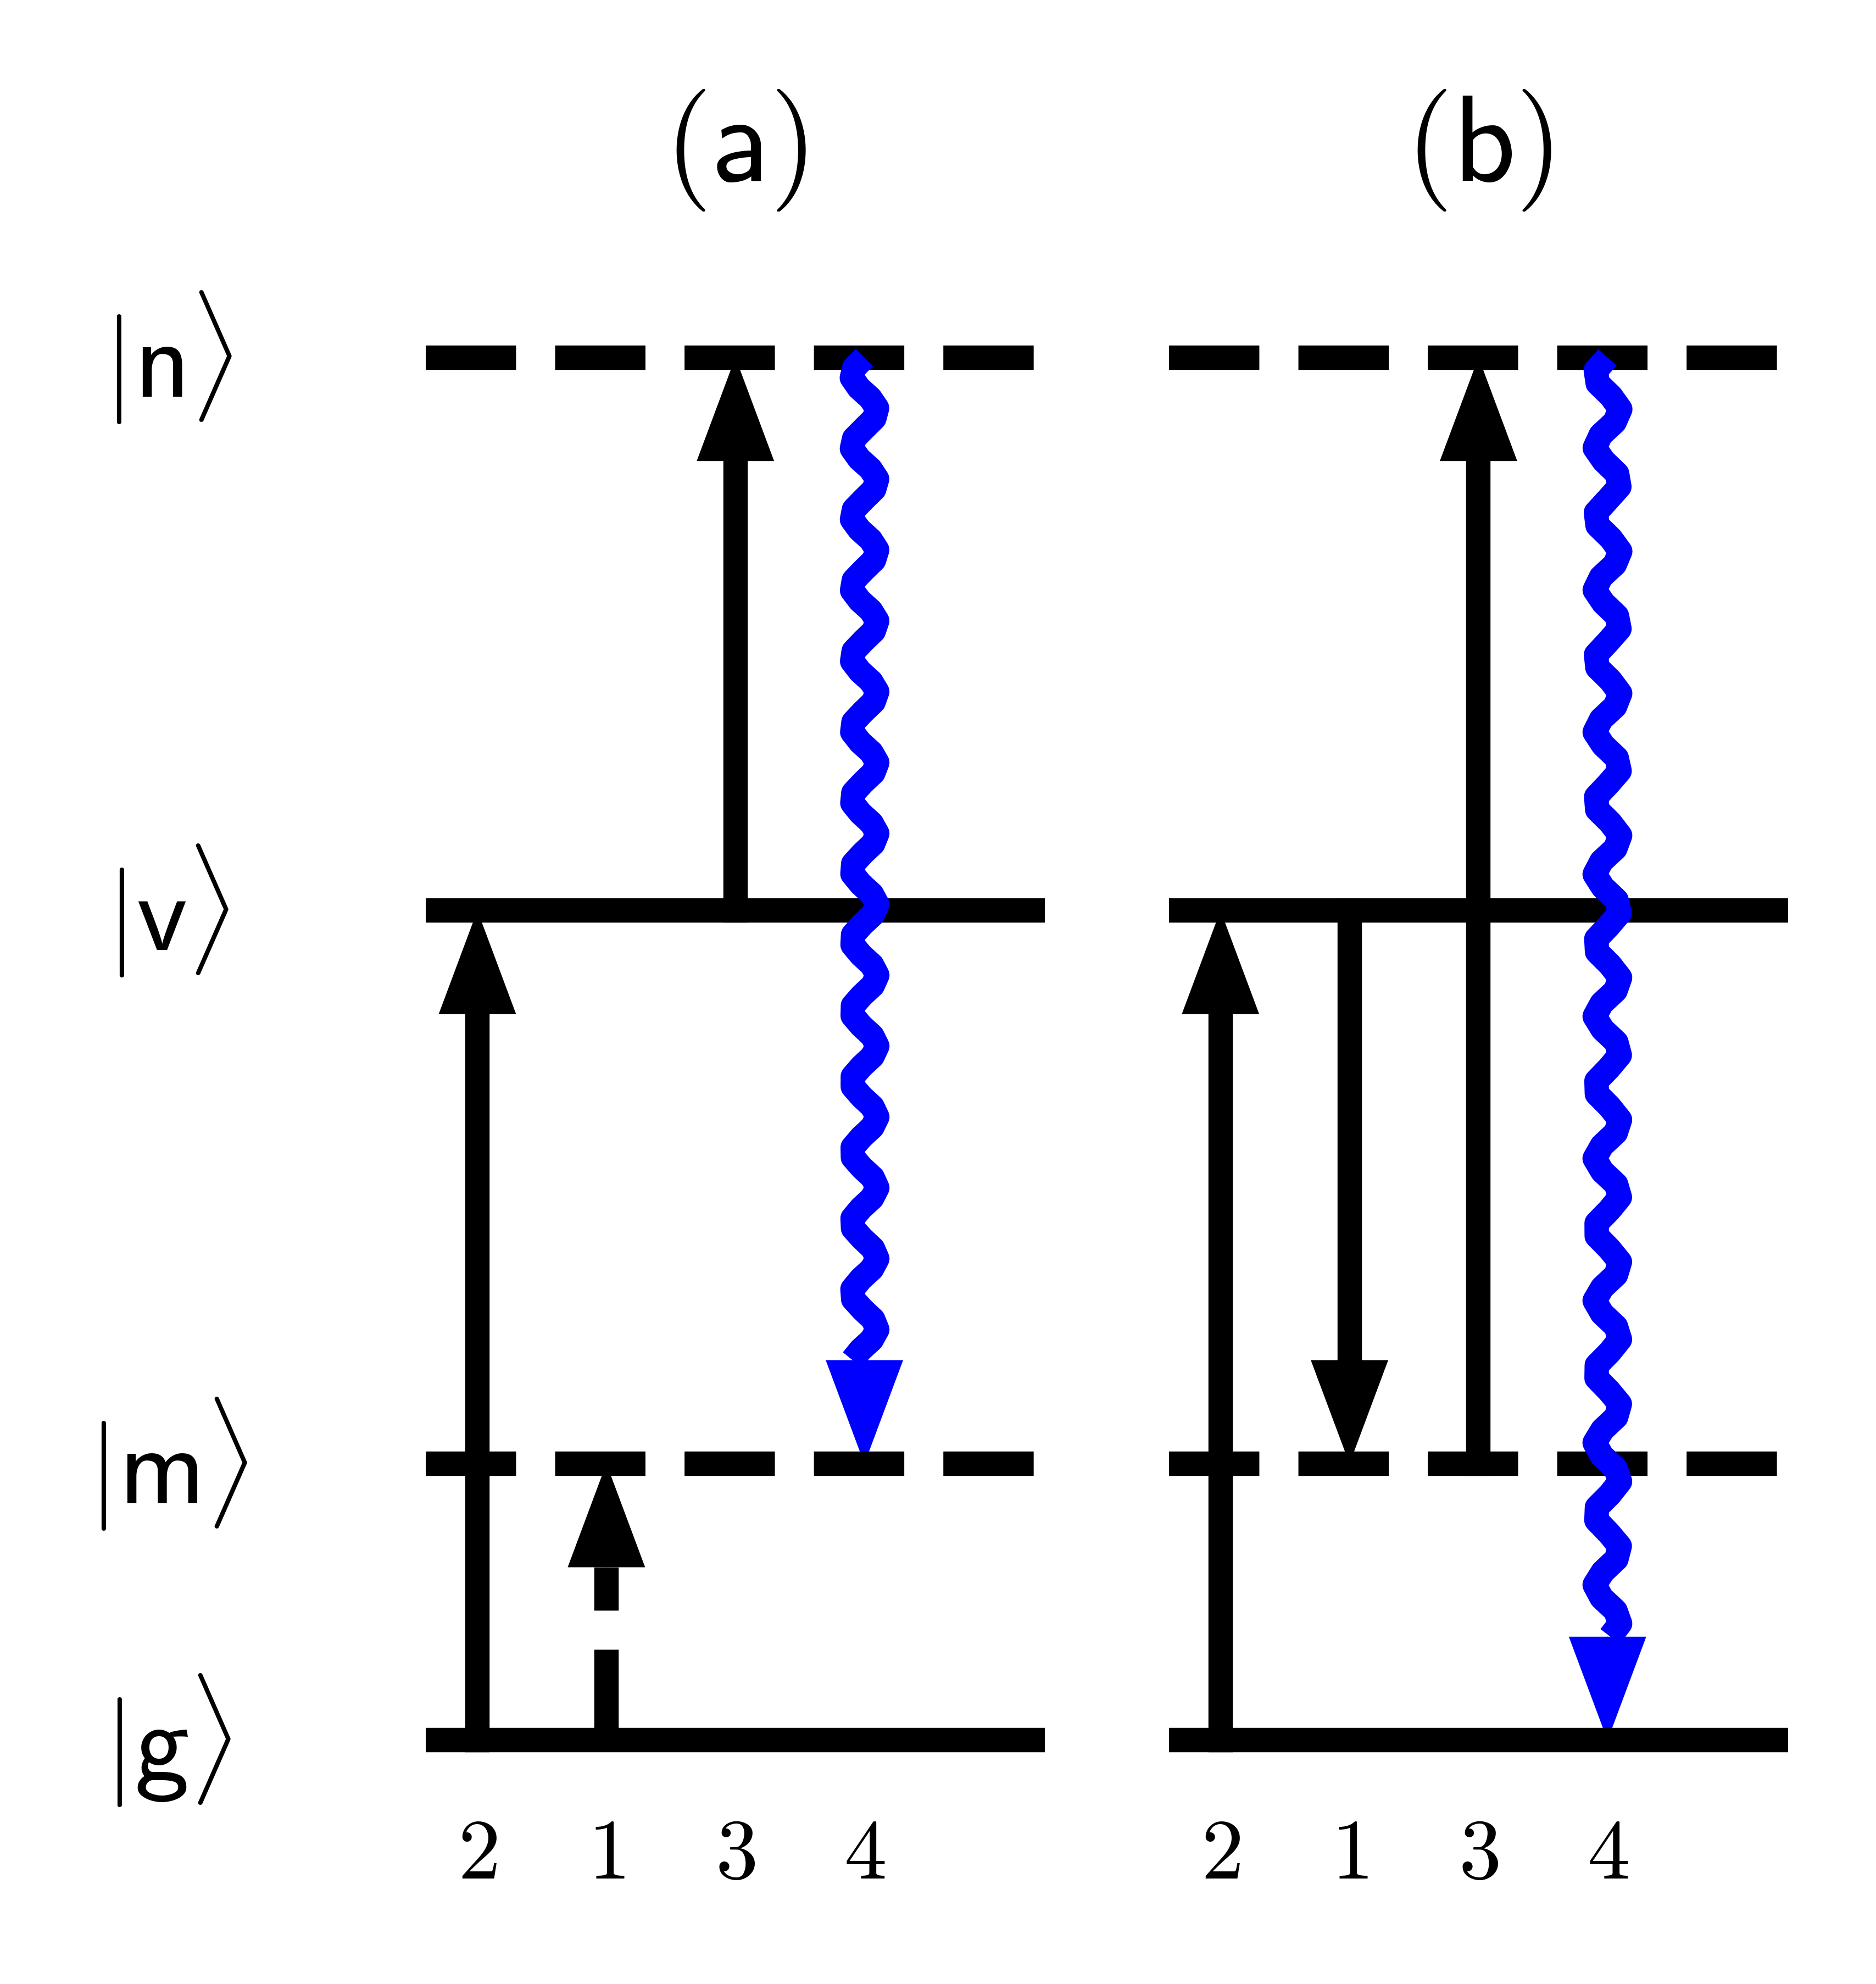
\includegraphics[width=3.375in]{figures/wmel2.png}
	\caption{Wave Mixing Energy Level (WMEL) diagrams of interfering hyper-DFG pathways in the  $\vec{k}_4 = -\vec{k}_1 + \vec{k}_2 + \vec{k}_3$ phasematching geometry. 
		(a) is similar to the process diagrammed in \autoref{fig:sivewmel}, whereas (b) is similar to a singly resonant coherent anti-Stokes Raman-type process.
		%todo: add pump-SIVE-probe to this set of WMELs
		}
	\label{fig:sivewmel2}
\end{figure}

We employ the response function formalism of Mukamel for this analysis. \cite{RN287}
The third order response functions, $R^{(3)}$, for \autoref{fig:sivewmel2}a ($R^{(3)}_{a}$) and \autoref{fig:sivewmel2}b ($R^{(3)}_{b}$) are 
\begin{subequations}
	\begin{equation} \label{mixing:a}
		R^{(3)}_{a} (t_2) = -\frac{i}{\hbar} [\beta(t_2), \mu(0)] \exp(-i\Delta_{v''g}t_2) \theta(t_2)
	\end{equation}
	\begin{equation}\label{mixing:b}
		\begin{split}
			R^{(3)}_{b} (t_2) & = \frac{i}{\hbar} [\beta(t_2), \mu(0)] \exp(-i\Delta_{v''g}t_2) \theta(t_2)\\
		\end{split}
	\end{equation}
\end{subequations}
The total response function is $R^{(3)}_\text{tot} (t_2) = R^{(3)}_{a} (t_2) + R^{(3)}_{b} (t_2) = 0$. 
Since the total output response function vanishes in this time-ordering, the pathways in \autoref{fig:sivewmel2} perfectly destructively interfere.
Therefore, to measure coherent dynamics via hyper-DFG, the time ordering shown in \autoref{fig:sivewmel} should be used.
These ideas have been seen experimentally in ultrafast DOVE work, as described elsewhere. \cite{RN367, McDonnell2024}
In the case of the time ordered (\autoref{fig:sivewmel}a) pathway, there are no opportunities for interference as all other pathways are nonresonant with the first interaction. 
A possible mechanism for interfering output in the (\autoref{fig:sivewmel}a) pathway are cascaded second order processes (SFG, DFG). \cite{RN243, RN300}
In isotropic media, SFG and DFG vanish under the electric dipole approximation,\cite{RN231} so cascades are unlikely to inhibit output in centrosymmetric media.
In media where SFG and DFG are allowed, e.g. surfaces or noncentrosymmetric media, second order cascades may become important. 


%todo: measuring Coherence and Population Lifetimes

\section{Experimental Hyper-DFG Results}
With the theoretical description of HDFG provided, we will investigate steady state and transient HDFG spectra of $\nu$(CH) modes in CH$_3$CN.

\subsection{dynamics} 
Look at coherence dynamics of v(CH), v(CN) in CH3CN. 
THIS EXPERIMENT IS DEFINITELY EASIER THAN EXTRACTING CHI3. 
 
\subsection{Calculation of $\beta$ for v(CH) modes in CH3CN}
do the classic C6D6 at CH3CN expt ? (or CaF2, whatever) - get interferogram, fit, get numbers.
Dipoles of CH3CN fitted by John in the 2003 paper, so only need to get $\beta$. 
Compare this to the theoretical CH3CN hyper Raman paper.
We can decide if this is worth it. 


\section{Conclusions}%didn't change to HDFG down here because lazy
Coherent vibrational, hyper-Raman coherent four wave mixing spectroscopies are identified and discussed.
Singly resonant SIVE (SR-SIVE) processes are shown to be the coherent hyper-Raman analogue of infrared active vibrations.
Since SR-SIVE is always non-zero for IR active vibrations, the method could be used as an analytical method to optically upconvert infrared transitions with small transition dipoles.
A method for measuring hyper-Raman polarizabilities, $\beta_{ijk}$, through SIVE spectroscopy was identified and discussed.
Extracting the magnitude and sign of $\beta_{ijk}$ using SIVE methods can help assess the quality of theoretical methods which calculate hyper-Raman spectra. 
Doubly resonant SIVE (DR-SIVE) processes show promise as a probe of vibronic coupling in molecular samples.
Unlike SR-SIVE, DR-SIVE methods can linenarrow inhomogeneously broadened vibronic modes. 

\section{Acknowledgments}
This work received support from the Department of Energy, Office of Basic Energy Sciences, Division of Materials Sciences and Engineering (Grant no. DE-SC0002162).
R.P.M. acknowledges support from the NSF Graduate Research Fellowship Program (Grant no. DGE-2137424). 


\section{References}
% Create the reference section using BibTeX:
\bibliography{library.bib}

\end{document}
%


